Tenemos la siguiente pila:
\begin{center}
    \begin{tabular}{|c|c|c|}
        \hline
        Estado actual & Siguientes estados y $f$ correspondientes & Cerrados\\
        \hline
        $s_0$ & $(s_2:5)$ & $s_0$ \\
        \hline
        $s_2$ & $(s_4:5), (s_1:7)$ & $s_0,s_2$ \\
        \hline
        $s_4$ & $(s_1:7), (s_3:9), (s_5:13)$ & $s_0,s_2,s_4$\\
        \hline
        $s_1$ & $(s_3:9), (s_5:13) $ & $ s_0,s_2,s_4, s_1$\\
        \hline
        $s_3$ & $(s_5:13) $ & $ s_0,s_2,s_4, s_1,s_3$\\
        \hline
        $s_5$ & $(s_5:12), (s_7:20) $ & $ s_0,s_2,s_4, s_1,s_3,s_5$\\
        \hline
        $s_6$ & $(s_7:17) $ & $ s_0,s_2,s_4, s_1,s_3,s_5,s_6$\\
        \hline
        $s_7$ & Estado final & $ s_0,s_2,s_4, s_1,s_3,s_5,s_6,s_7$\\
        \hline
    \end{tabular}
\end{center}
Se tiene el siguiente árbol:
\begin{center}
    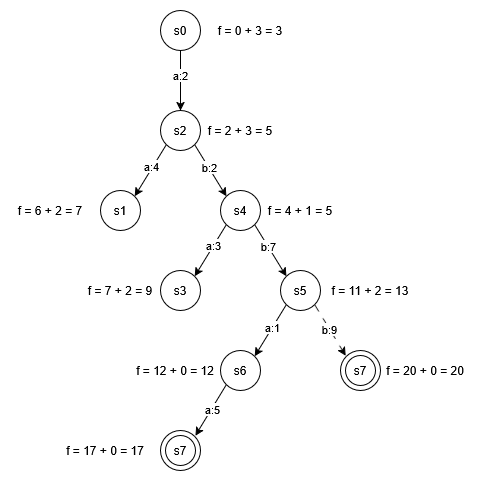
\includegraphics[height = 10cm]{respuestas/img/treeE7d.png}
\end{center}
Por lo que el camino solución es $a,b,b,a,a$, conformado por los estados $s_0,s_2,s_4,s_5,s_6,s_7$.